%
\hsection{Virtual Environments in PyCharm}%
%
\begin{figure}%
\centering%
%
\subfloat[][%
We create a new project in \pycharm\ and select a \pgls{virtualEnvironment} as \menu{Custom Environment}. %
We click~\menu{Create}.%
\label{fig:venvPycharm1}%
]{\tightbox{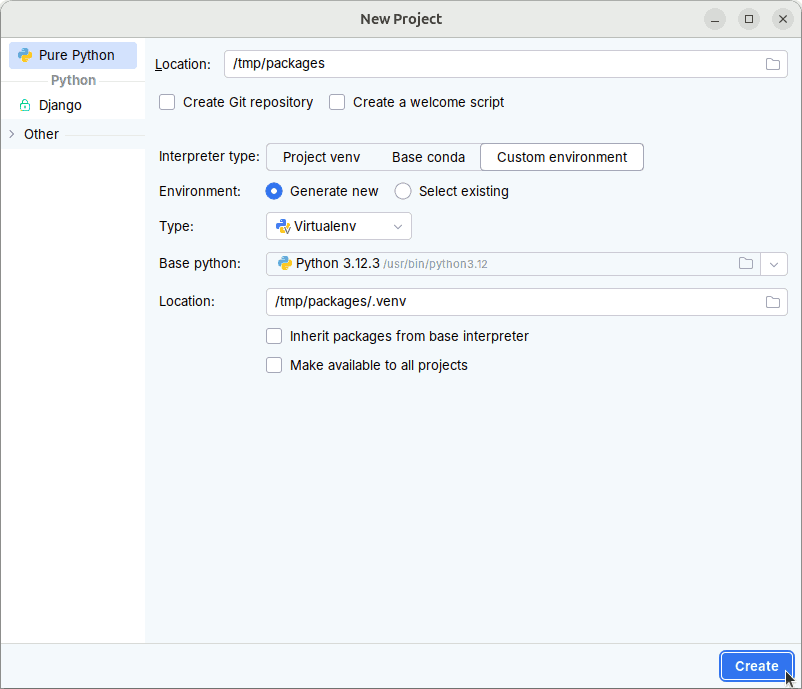
\includegraphics[width=0.48\linewidth]{\currentDir/venvPycharm1}}}%
%
\floatSep%
%
\subfloat[][%
Since I selected the folder where the other files (\textil{requirements.txt}, \textil{numpy_user.py}, \dots) are already located, \pycharm\ asks whether this is OK. %
We select \menu{Create from Existing Sources} if asked.%
\label{fig:venvPycharm2}%
]{\tightbox{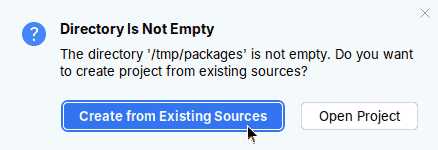
\includegraphics[width=0.48\linewidth]{\currentDir/venvPycharm2}}}%
%
\floatRowSep%
%
\subfloat[][%
Let's take a look at \textil{requirements.txt}. %
We double-click on this file.%
\label{fig:venvPycharm3}%
]{\tightbox{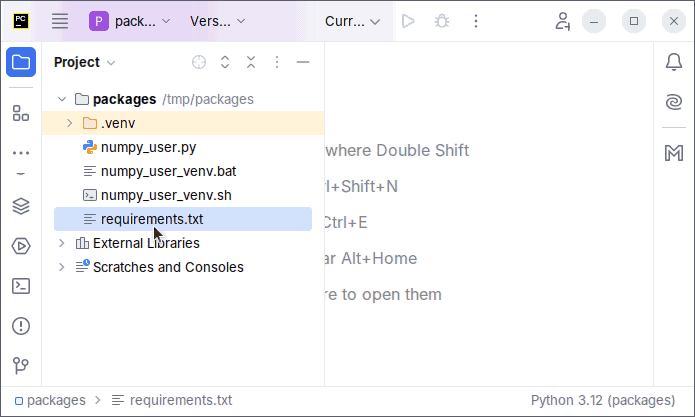
\includegraphics[width=0.48\linewidth]{\currentDir/venvPycharm3}}}%
%
\floatSep%
%
\subfloat[][%
It contains the one line \textil{numpy==1.26.4}, which means that our project requires \numpy\ in version~1.26.4.%
\label{fig:venvPycharm4}%
]{\tightbox{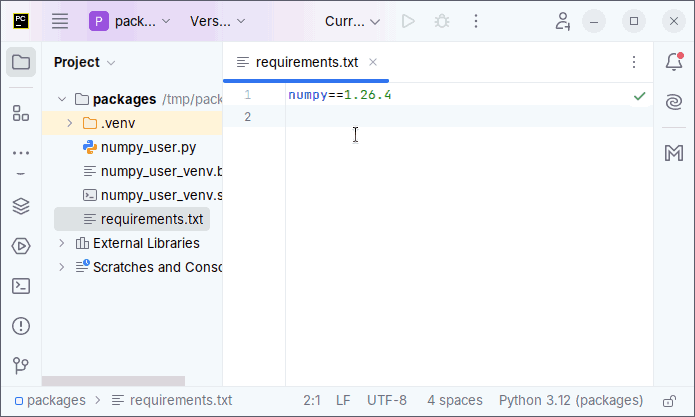
\includegraphics[width=0.48\linewidth]{\currentDir/venvPycharm4}}}%
%
%
\caption{Using \textil{requirements.txt} and \pglspl{virtualEnvironment} in \pycharm~(part~1).}%
\label{fig:venvPycharmA}%
\end{figure}%
%
\begin{figure}%
\ContinuedFloat%
\centering%
%
\subfloat[][%
We now click on \textil{numpy_user.py} and get informed that required \pglspl{package} are missing. %
We can install them into our project's \pgls{virtualEnvironment} by clicking \menu{Install requirement}. %
Notice:~This question could also have popped up when we opened \textil{requirements.txt}, in which case we would have installed the requirements then.%
\label{fig:venvPycharm5}%
]{\tightbox{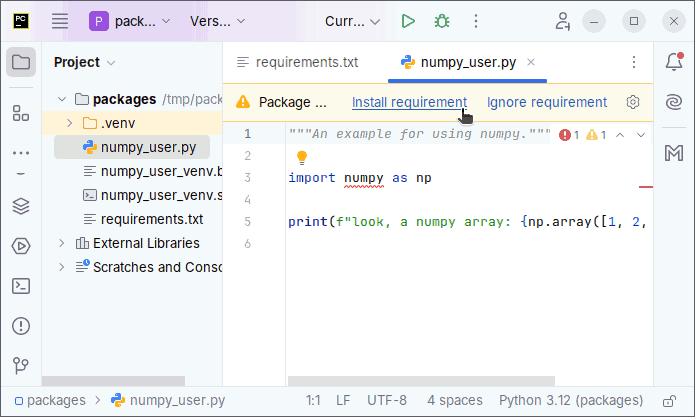
\includegraphics[width=0.48\linewidth]{\currentDir/venvPycharm5}}}%
%
\floatSep%
%
\subfloat[][%
We get informed that the required packages were successfully installed.%
\label{fig:venvPycharm6}%
]{\tightbox{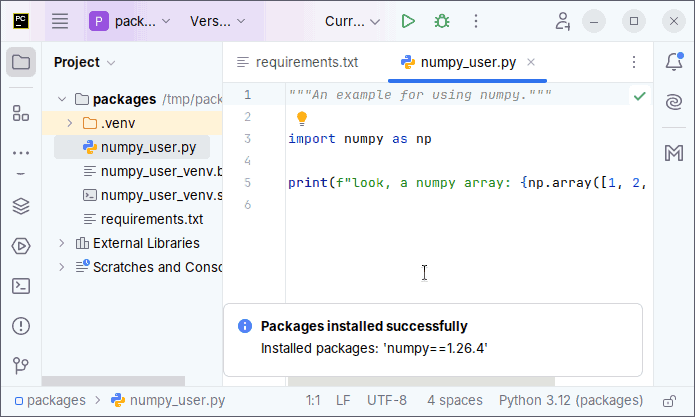
\includegraphics[width=0.48\linewidth]{\currentDir/venvPycharm6}}}%
%
\floatRowSep%
%
\subfloat[][%
We right-click on \textil{numpy_user.py} and click on~\menu{Run \inSQuotes{numpy\_user.py}}.%
\label{fig:venvPycharm7}%
]{\tightbox{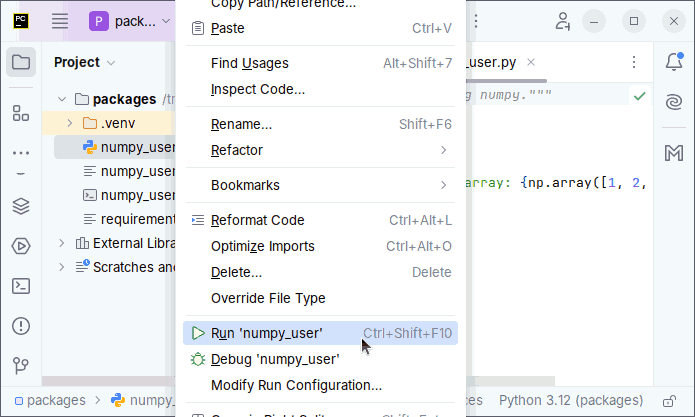
\includegraphics[width=0.48\linewidth]{\currentDir/venvPycharm7}}}%
%
\floatSep%
%
\subfloat[][%
Our program is executed without error and produces the expected output.%
\label{fig:venvPycharm8}%
]{\tightbox{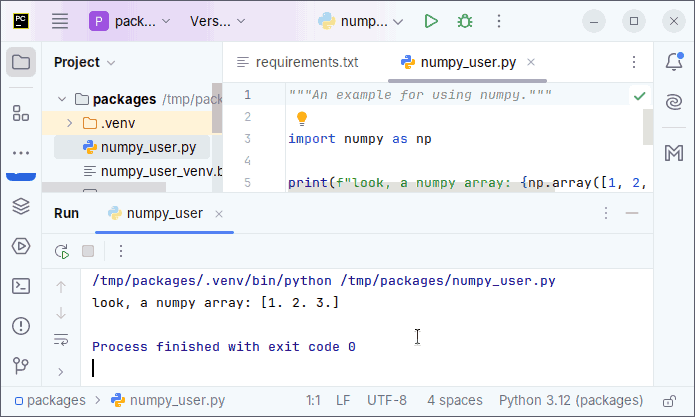
\includegraphics[width=0.48\linewidth]{\currentDir/venvPycharm8}}}%
%
%
\caption{Using \textil{requirements.txt} and \pglspl{virtualEnvironment} in \pycharm~(part~2).}%
\label{fig:venvPycharmB}%
\end{figure}%
%
The \pgls{IDE} \pycharm\ also supports using \pglspl{virtualEnvironment} and \textil{requirements.txt} files.
Let us here demonstrate this on the example program that requires \numpy\ which was given as \cref{lst:packages:numpy_user} and \textil{requirements.txt} file given in \cref{lst:packages:requirementstxt}.
In \cref{fig:venvPycharmA}, we work through the steps to create and manage a project with a \pgls{virtualEnvironment} in \pycharm\ on their basis.

First, we need to create a new project~(\cref{fig:venvPycharm1}).
For this purpose, we already copied the files \pglspl{virtualEnvironment} and \textil{requirements.txt} into a folder~(here:~\textil{/tmp/packages}).
In the \menu{New Project} dialog of \pycharm, we select this folder as \menu{Location:}.
As \menu{Interpreter type:}, we choose \menu{Custom Environment} and as \menu{Environment:}, we pick \menu{Generate new}.
As \menu{Type:}, we choose \menu{Virtualenv}.
The default \menu{Location} is \textil{.venv} inside our project directory and we keep this setting.
After clicking \menu{Create}, a new project is created.

Well, almost:
\Cref{fig:venvPycharm2} reminds me that I copied some files into the project folder before creating the project.
\pycharm\ wants to make sure that this is right and asks me so.
As answer, I click~\menu{Create from Existing Sources}.

We now are in the normal \pycharm\ project view in~\cref{fig:venvPycharm3}.
All the files that I placed into the folder are there and also a \textil{.venv} directory has been created.
Notice that you could as well create an empty project and copy the files there.

We click on \textil{requirements.txt} and it opens in~\cref{fig:venvPycharm4}.
Indeed, the file prescribes a single requirement, \numpy\ in version~1.26.4.

When we click on the file \textil{numpy_user.py} to open it in~\cref{fig:venvPycharm5}, we notice a yellow bar at the top of the file's contents.
This bar tells us that the required package \numpy\ is missing.
It offers us the two choices to either \menu{Install requirement} or to \menu{Ignore requirement}.
We select the first option and click it.
Notice that this same yellow bar could also have appeared when we opened \textil{requirements.txt}.
I am not sure why it appears only now.
Either way, we accept the choice to install the requirement.

In \cref{fig:venvPycharm6}, we are informed that the installation was successful.
The small overlay also tells us that \numpy\ was installed in version~1.26.4, as prescribed by the \textil{requirements.txt} file.
At the time of this writing, \numpy\ is already out at version~2.2.1, which would have been used if we had just installed it without version specification.
So this confirms that, indeed, our \textil{requirements.txt} is used.
We also can see that the red underline under \pythonilIdx{numpy} that was present in \cref{fig:venvPycharm5} is now gone in \cref{fig:venvPycharm6}, because now the package and corresponding modules can be loaded without error.

As final check that everything went well we run our program \textil{numpy_user.py} in \cref{fig:venvPycharm7}.
We right-click the file in three view on the left-hand side of the window.
A popup menu appears, in which we click on \menu{Run \inSQuotes{numpy\_user.py}}.
We could just as well have pressed \keys{\ctrl+\shift+F10}.
Our program is executed and the expected output appears (\cref{fig:venvPycharm8}).
All is well.

However, it must be understood that the support for \pglspl{virtualEnvironment} and requirements files in \pycharm\ is for \emph{software development}.
If you want to actually use the software you have developed, you should \emph{always} use the command line and \pglspl{terminal}, as discussed in \cref{sec:pipAndVenv}.
\pycharm\ is not a runtime environment for the deployment of productive code.
It is an \acrfull{IDE} for developing programs.%
%
\bestPractice{noPycharmForProductive}{%
\pycharm\ must \textbf{never} be used for running an application in a productive setting. %
It is \emph{only} to be used as \pgls{IDE} for software development. %
For actually executing programs, always use a \pglspl{virtualEnvironment} in the \pgls{terminal} as introduced in \cref{sec:pipAndVenv}. %
See also \cref{bp:runningProgram}.%
}%
%
This holds also and especially for scenarios where we do use \python\ for scientific experiments.
It is an even worse idea to try to run multiple concurrent instances of a program in a \pycharm\ window or to have multiple \pycharm\ instances open to run multiple applications in parallel.%
%
\FloatBarrier%
\endhsection%
%
